\documentclass[9pt,letter]{article}
\usepackage{lmodern}
\usepackage{amssymb,amsmath}
\usepackage{ifxetex,ifluatex}
\usepackage{fixltx2e} % provides \textsubscript
\ifnum 0\ifxetex 1\fi\ifluatex 1\fi=0 % if pdftex
  \usepackage[T1]{fontenc}
  \usepackage[utf8]{inputenc}
\else % if luatex or xelatex
  \ifxetex
    \usepackage{mathspec}
  \else
    \usepackage{fontspec}
  \fi
  \defaultfontfeatures{Ligatures=TeX,Scale=MatchLowercase}
\fi
% use upquote if available, for straight quotes in verbatim environments
\IfFileExists{upquote.sty}{\usepackage{upquote}}{}
% use microtype if available
\IfFileExists{microtype.sty}{%
\usepackage{microtype}
\UseMicrotypeSet[protrusion]{basicmath} % disable protrusion for tt fonts
}{}
\usepackage[margin=.75in]{geometry}
\usepackage{hyperref}
\hypersetup{unicode=true,
            pdftitle={Assignment 4},
            pdfauthor={Azoacha Forcheh, 20558994},
            pdfborder={0 0 0},
            breaklinks=true}
\urlstyle{same}  % don't use monospace font for urls
\usepackage{color}
\usepackage{fancyvrb}
\newcommand{\VerbBar}{|}
\newcommand{\VERB}{\Verb[commandchars=\\\{\}]}
\DefineVerbatimEnvironment{Highlighting}{Verbatim}{commandchars=\\\{\}}
% Add ',fontsize=\small' for more characters per line
\usepackage{framed}
\definecolor{shadecolor}{RGB}{248,248,248}
\newenvironment{Shaded}{\begin{snugshade}}{\end{snugshade}}
\newcommand{\KeywordTok}[1]{\textcolor[rgb]{0.13,0.29,0.53}{\textbf{#1}}}
\newcommand{\DataTypeTok}[1]{\textcolor[rgb]{0.13,0.29,0.53}{#1}}
\newcommand{\DecValTok}[1]{\textcolor[rgb]{0.00,0.00,0.81}{#1}}
\newcommand{\BaseNTok}[1]{\textcolor[rgb]{0.00,0.00,0.81}{#1}}
\newcommand{\FloatTok}[1]{\textcolor[rgb]{0.00,0.00,0.81}{#1}}
\newcommand{\ConstantTok}[1]{\textcolor[rgb]{0.00,0.00,0.00}{#1}}
\newcommand{\CharTok}[1]{\textcolor[rgb]{0.31,0.60,0.02}{#1}}
\newcommand{\SpecialCharTok}[1]{\textcolor[rgb]{0.00,0.00,0.00}{#1}}
\newcommand{\StringTok}[1]{\textcolor[rgb]{0.31,0.60,0.02}{#1}}
\newcommand{\VerbatimStringTok}[1]{\textcolor[rgb]{0.31,0.60,0.02}{#1}}
\newcommand{\SpecialStringTok}[1]{\textcolor[rgb]{0.31,0.60,0.02}{#1}}
\newcommand{\ImportTok}[1]{#1}
\newcommand{\CommentTok}[1]{\textcolor[rgb]{0.56,0.35,0.01}{\textit{#1}}}
\newcommand{\DocumentationTok}[1]{\textcolor[rgb]{0.56,0.35,0.01}{\textbf{\textit{#1}}}}
\newcommand{\AnnotationTok}[1]{\textcolor[rgb]{0.56,0.35,0.01}{\textbf{\textit{#1}}}}
\newcommand{\CommentVarTok}[1]{\textcolor[rgb]{0.56,0.35,0.01}{\textbf{\textit{#1}}}}
\newcommand{\OtherTok}[1]{\textcolor[rgb]{0.56,0.35,0.01}{#1}}
\newcommand{\FunctionTok}[1]{\textcolor[rgb]{0.00,0.00,0.00}{#1}}
\newcommand{\VariableTok}[1]{\textcolor[rgb]{0.00,0.00,0.00}{#1}}
\newcommand{\ControlFlowTok}[1]{\textcolor[rgb]{0.13,0.29,0.53}{\textbf{#1}}}
\newcommand{\OperatorTok}[1]{\textcolor[rgb]{0.81,0.36,0.00}{\textbf{#1}}}
\newcommand{\BuiltInTok}[1]{#1}
\newcommand{\ExtensionTok}[1]{#1}
\newcommand{\PreprocessorTok}[1]{\textcolor[rgb]{0.56,0.35,0.01}{\textit{#1}}}
\newcommand{\AttributeTok}[1]{\textcolor[rgb]{0.77,0.63,0.00}{#1}}
\newcommand{\RegionMarkerTok}[1]{#1}
\newcommand{\InformationTok}[1]{\textcolor[rgb]{0.56,0.35,0.01}{\textbf{\textit{#1}}}}
\newcommand{\WarningTok}[1]{\textcolor[rgb]{0.56,0.35,0.01}{\textbf{\textit{#1}}}}
\newcommand{\AlertTok}[1]{\textcolor[rgb]{0.94,0.16,0.16}{#1}}
\newcommand{\ErrorTok}[1]{\textcolor[rgb]{0.64,0.00,0.00}{\textbf{#1}}}
\newcommand{\NormalTok}[1]{#1}
\usepackage{graphicx,grffile}
\makeatletter
\def\maxwidth{\ifdim\Gin@nat@width>\linewidth\linewidth\else\Gin@nat@width\fi}
\def\maxheight{\ifdim\Gin@nat@height>\textheight\textheight\else\Gin@nat@height\fi}
\makeatother
% Scale images if necessary, so that they will not overflow the page
% margins by default, and it is still possible to overwrite the defaults
% using explicit options in \includegraphics[width, height, ...]{}
\setkeys{Gin}{width=\maxwidth,height=\maxheight,keepaspectratio}
\IfFileExists{parskip.sty}{%
\usepackage{parskip}
}{% else
\setlength{\parindent}{0pt}
\setlength{\parskip}{6pt plus 2pt minus 1pt}
}
\setlength{\emergencystretch}{3em}  % prevent overfull lines
\providecommand{\tightlist}{%
  \setlength{\itemsep}{0pt}\setlength{\parskip}{0pt}}
\setcounter{secnumdepth}{0}
% Redefines (sub)paragraphs to behave more like sections
\ifx\paragraph\undefined\else
\let\oldparagraph\paragraph
\renewcommand{\paragraph}[1]{\oldparagraph{#1}\mbox{}}
\fi
\ifx\subparagraph\undefined\else
\let\oldsubparagraph\subparagraph
\renewcommand{\subparagraph}[1]{\oldsubparagraph{#1}\mbox{}}
\fi

%%% Use protect on footnotes to avoid problems with footnotes in titles
\let\rmarkdownfootnote\footnote%
\def\footnote{\protect\rmarkdownfootnote}

%%% Change title format to be more compact
\usepackage{titling}

% Create subtitle command for use in maketitle
\newcommand{\subtitle}[1]{
  \posttitle{
    \begin{center}\large#1\end{center}
    }
}

\setlength{\droptitle}{-2em}
  \title{Assignment 4}
  \pretitle{\vspace{\droptitle}\centering\huge}
  \posttitle{\par}
  \author{Azoacha Forcheh, 20558994}
  \preauthor{\centering\large\emph}
  \postauthor{\par}
  \date{}
  \predate{}\postdate{}

\usepackage{graphicx}
\usepackage{color}
\usepackage{enumitem}
\newcommand{\benum}{\begin{enumerate}}
\newcommand{\eenum}{\end{enumerate}}
\newcommand{\bitem}{\begin{itemize}}
\newcommand{\eitem}{\end{itemize}}

\begin{document}
\maketitle

\benum
\item  \textbf{Antarctic sea ice} On the website for this assignment, in
the directory called \texttt{R} you will find a file called
\texttt{seaice.csv}. Download this file.

We will need to do some manipulations to this data before it can be
easily used in our analysis.

\begin{Shaded}
\begin{Highlighting}[]
\NormalTok{seaice <-}\StringTok{ }\KeywordTok{read.csv}\NormalTok{(}\StringTok{"./R/seaice.csv"}\NormalTok{, }\DataTypeTok{header=}\OtherTok{TRUE}\NormalTok{)}
\end{Highlighting}
\end{Shaded}

The last line above shows that \texttt{seaice} is a data frame having
four variates. The first three identify the year, month, and day that
the last measurement was taken. The last measure is a determination of
the extent of Antarctic sea ice in millions of square kilometres as
determined by satellite imagery.

\benum
\item *Irregular time series* First, we begin by putting the year,
month, and day together into a single date. Do this as follows:

\begin{Shaded}
\begin{Highlighting}[]
\NormalTok{date <-}\StringTok{ }\KeywordTok{paste}\NormalTok{(seaice}\OperatorTok{$}\NormalTok{Year,seaice}\OperatorTok{$}\NormalTok{Month,seaice}\OperatorTok{$}\NormalTok{Day, }\DataTypeTok{sep=}\StringTok{" "}\NormalTok{)}
\KeywordTok{head}\NormalTok{(date)}
\end{Highlighting}
\end{Shaded}

\begin{verbatim}
## [1] "1979 1 2"  "1979 1 4"  "1979 1 6"  "1979 1 8"  "1979 1 10" "1979 1 12"
\end{verbatim}

\begin{Shaded}
\begin{Highlighting}[]
\CommentTok{# The following function turns that into a standard date format}
\CommentTok{# You will need the package "lubridate"}
\KeywordTok{library}\NormalTok{(lubridate)}
\end{Highlighting}
\end{Shaded}

\begin{verbatim}
## 
## Attaching package: 'lubridate'
\end{verbatim}

\begin{verbatim}
## The following object is masked from 'package:base':
## 
##     date
\end{verbatim}

\begin{Shaded}
\begin{Highlighting}[]
\NormalTok{date <-}\StringTok{ }\KeywordTok{ymd}\NormalTok{(date)}
\KeywordTok{head}\NormalTok{(date)}
\end{Highlighting}
\end{Shaded}

\begin{verbatim}
## [1] "1979-01-02" "1979-01-04" "1979-01-06" "1979-01-08" "1979-01-10"
## [6] "1979-01-12"
\end{verbatim}

\begin{Shaded}
\begin{Highlighting}[]
\CommentTok{# And we create a new data structure called sea.ice}
\NormalTok{sea.ice <-}\StringTok{ }\KeywordTok{data.frame}\NormalTok{(}\DataTypeTok{date=}\NormalTok{date, }\DataTypeTok{extent =}\NormalTok{ seaice}\OperatorTok{$}\NormalTok{Extent)}
\KeywordTok{head}\NormalTok{(sea.ice)}
\end{Highlighting}
\end{Shaded}

\begin{verbatim}
##         date extent
## 1 1979-01-02  6.945
## 2 1979-01-04  6.841
## 3 1979-01-06  6.648
## 4 1979-01-08  6.270
## 5 1979-01-10  6.138
## 6 1979-01-12  5.957
\end{verbatim}

We will be using the data frame \texttt{sea.ice} for this part of the
question.

\benum
\item  \textbf{(4 marks)} Call \texttt{plot(...)} directly on the data
frame \texttt{sea.ice} with \texttt{cex=0.3,\ pch=19,\ col="darkgrey"}.
Zoom in on this plot and experiment with different aspect ratios by
reshaping the plot's window. Describe whatever interesting
characteristics you see in the time series.

\begin{Shaded}
\begin{Highlighting}[]
\CommentTok{# Aspect ratio}
\NormalTok{savePar =}\StringTok{ }\KeywordTok{par}\NormalTok{(}\DataTypeTok{mfrow=}\KeywordTok{c}\NormalTok{(}\DecValTok{2}\NormalTok{,}\DecValTok{3}\NormalTok{), }\DataTypeTok{mar=}\KeywordTok{c}\NormalTok{(}\FloatTok{2.5}\NormalTok{,}\FloatTok{0.1}\NormalTok{,}\DecValTok{3}\NormalTok{,}\FloatTok{0.1}\NormalTok{))}
\KeywordTok{plot}\NormalTok{(sea.ice, }\DataTypeTok{xlab=}\StringTok{""}\NormalTok{, }\DataTypeTok{ylab=}\StringTok{""}\NormalTok{, }\DataTypeTok{axes=}\OtherTok{FALSE}\NormalTok{,}
     \DataTypeTok{main=}\StringTok{"Original Plot"}\NormalTok{, }\DataTypeTok{cex=}\FloatTok{0.3}\NormalTok{, }\DataTypeTok{pch=}\DecValTok{19}\NormalTok{, }\DataTypeTok{col=}\StringTok{"darkgrey"}\NormalTok{)}
\ControlFlowTok{for}\NormalTok{ (aspect }\ControlFlowTok{in} \KeywordTok{c}\NormalTok{(}\DecValTok{400}\NormalTok{, }\DecValTok{200}\NormalTok{, }\DecValTok{500}\NormalTok{, }\DecValTok{600}\NormalTok{)) \{}
  \KeywordTok{plot}\NormalTok{(sea.ice, }\DataTypeTok{asp=}\NormalTok{aspect,}
       \DataTypeTok{main=}\KeywordTok{paste}\NormalTok{(}\StringTok{"aspect ="}\NormalTok{,aspect),}
       \DataTypeTok{xlab=}\StringTok{""}\NormalTok{, }\DataTypeTok{ylab=}\StringTok{""}\NormalTok{, }\DataTypeTok{axes=}\OtherTok{FALSE}\NormalTok{,}
       \DataTypeTok{cex=}\FloatTok{0.3}\NormalTok{, }\DataTypeTok{pch=}\DecValTok{19}\NormalTok{, }\DataTypeTok{col=}\StringTok{"darkgrey"}\NormalTok{)}
\NormalTok{\}}
\KeywordTok{par}\NormalTok{(savePar)}
\end{Highlighting}
\end{Shaded}

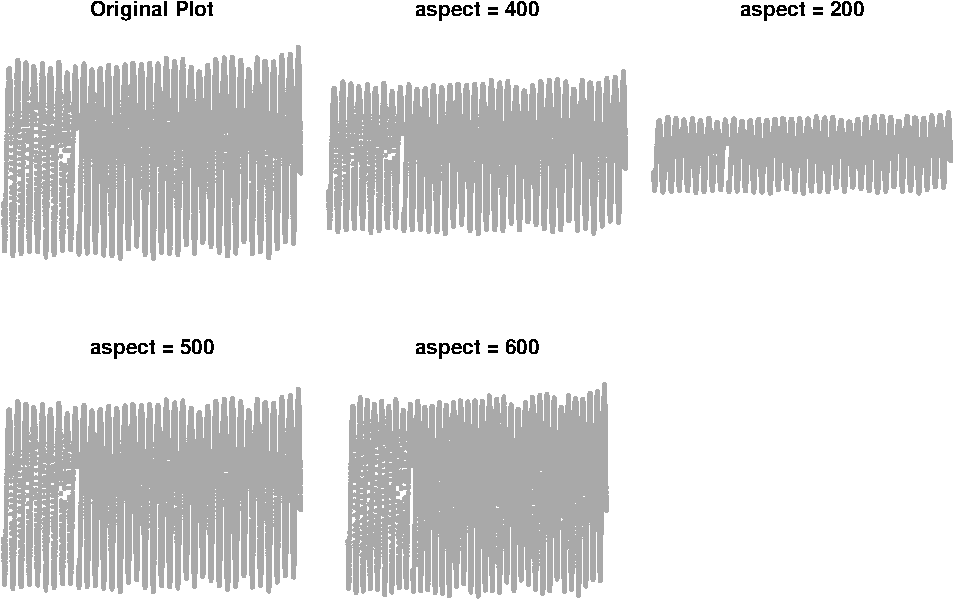
\includegraphics{a4_q3_files/figure-latex/unnamed-chunk-3-1.pdf}

\begin{Shaded}
\begin{Highlighting}[]
\CommentTok{# Zooming with loon}
\KeywordTok{require}\NormalTok{(loon)}
\end{Highlighting}
\end{Shaded}

\begin{verbatim}
## Loading required package: loon
\end{verbatim}

\begin{verbatim}
## Loading required package: tcltk
\end{verbatim}

\begin{Shaded}
\begin{Highlighting}[]
\KeywordTok{l_plot}\NormalTok{(sea.ice, }\DataTypeTok{showScales=}\OtherTok{TRUE}\NormalTok{, }
     \DataTypeTok{size=}\FloatTok{0.3}\NormalTok{, }\DataTypeTok{glyph=}\StringTok{"ccircle"}\NormalTok{, }
     \DataTypeTok{color=}\StringTok{"darkgrey"}\NormalTok{)}
\end{Highlighting}
\end{Shaded}

\begin{verbatim}
## [1] ".l0.plot"
## attr(,"class")
## [1] "loon"
\end{verbatim}

The value of the extent of the Antartic sea ice stays within the same
range, but it continuously sharply decreasing and increasing over short
time periods.

\item 

Decomposition into a long term trend and a short term trend. First we
need to transform the data again.

\begin{Shaded}
\begin{Highlighting}[]
\NormalTok{sea.ice.xy <-}\StringTok{ }\KeywordTok{xy.coords}\NormalTok{(sea.ice)}
\NormalTok{y <-}\StringTok{ }\NormalTok{sea.ice.xy}\OperatorTok{$}\NormalTok{y}
\NormalTok{x <-}\StringTok{ }\NormalTok{sea.ice.xy}\OperatorTok{$}\NormalTok{x}
\CommentTok{# plotting x and y as before will yield the same plot, but}
\CommentTok{# with the dates lost.}
\CommentTok{#plot(x, y, cex=0.3, pch=19, col="darkgrey")}
\end{Highlighting}
\end{Shaded}

The data range from the beginning of 1979 to the end of 2014. The number
of years covered then is (2014-1979 + 1)=36. So each year is
approximately 1/36 of the series. A month is about 1/12 of this again.

\bitem    \item \textbf{(2 marks)} Using \texttt{loess(..)} as in class,
find a long term trend using \texttt{span=2/3}. Add this trend as a
curve in a different colour on top the points (as in the above plot).
Describe the fit.

\begin{Shaded}
\begin{Highlighting}[]
\NormalTok{ltfit =}\StringTok{ }\KeywordTok{loess}\NormalTok{(y}\OperatorTok{~}\NormalTok{x, }\DataTypeTok{span=}\DecValTok{2}\OperatorTok{/}\DecValTok{3}\NormalTok{)}
\NormalTok{ltpred =}\StringTok{ }\KeywordTok{predict}\NormalTok{(ltfit)}
\NormalTok{xord =}\StringTok{ }\KeywordTok{order}\NormalTok{(x)}
\KeywordTok{plot}\NormalTok{(x, y, }\DataTypeTok{col=}\StringTok{"grey70"}\NormalTok{, }\DataTypeTok{pch=}\DecValTok{19}\NormalTok{, }
     \DataTypeTok{main=}\StringTok{"Locating the Long Term Trend"}\NormalTok{)}
\KeywordTok{lines}\NormalTok{(x[xord], ltpred[xord], }\DataTypeTok{lwd=}\DecValTok{2}\NormalTok{, }\DataTypeTok{col=}\StringTok{"steelblue"}\NormalTok{)}
\end{Highlighting}
\end{Shaded}

\begin{center}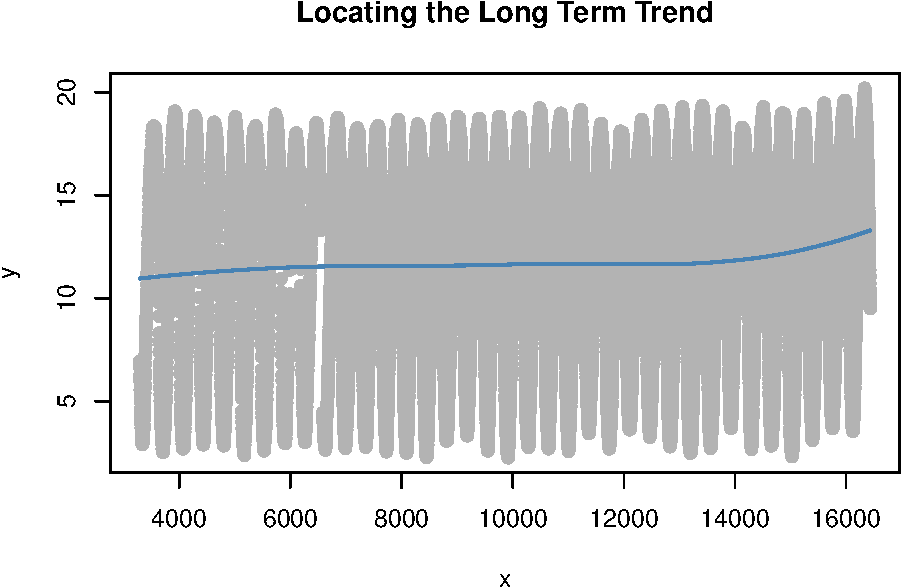
\includegraphics{a4_q3_files/figure-latex/unnamed-chunk-6-1} \end{center}

The extent of Antarctic sea ice stays fairly consistent and stationary,
then there is a small jump upwards and the extent begins to trend
upwards (i.e.~increase) slowly.

\item 

\textbf{(2 marks)} Now fit a \texttt{loess} short term smooth with
\texttt{span=1/(36*12)} to the residuals from the long term trend. Plot
the residuals from the long-term trend and add the fitted short term
trend. Describe the fit.

\begin{Shaded}
\begin{Highlighting}[]
\NormalTok{resids =}\StringTok{ }\NormalTok{ltfit}\OperatorTok{$}\NormalTok{residuals}
\KeywordTok{plot}\NormalTok{(x, resids, }\DataTypeTok{col=}\StringTok{"grey70"}\NormalTok{, }\DataTypeTok{pch=}\DecValTok{19}\NormalTok{, }
     \DataTypeTok{main=}\StringTok{"Small Fit of Residuals from Long Term Trend"}\NormalTok{)}
\NormalTok{smfit =}\StringTok{ }\KeywordTok{loess}\NormalTok{(resids}\OperatorTok{~}\NormalTok{x, }\DataTypeTok{span=}\DecValTok{1}\OperatorTok{/}\NormalTok{(}\DecValTok{36}\OperatorTok{*}\DecValTok{12}\NormalTok{))}
\NormalTok{smpred =}\StringTok{ }\KeywordTok{predict}\NormalTok{(smfit)}
\KeywordTok{lines}\NormalTok{(x[xord], smpred[xord], }\DataTypeTok{lwd=}\DecValTok{2}\NormalTok{, }\DataTypeTok{col=}\StringTok{"steelblue"}\NormalTok{)}
\end{Highlighting}
\end{Shaded}

\begin{center}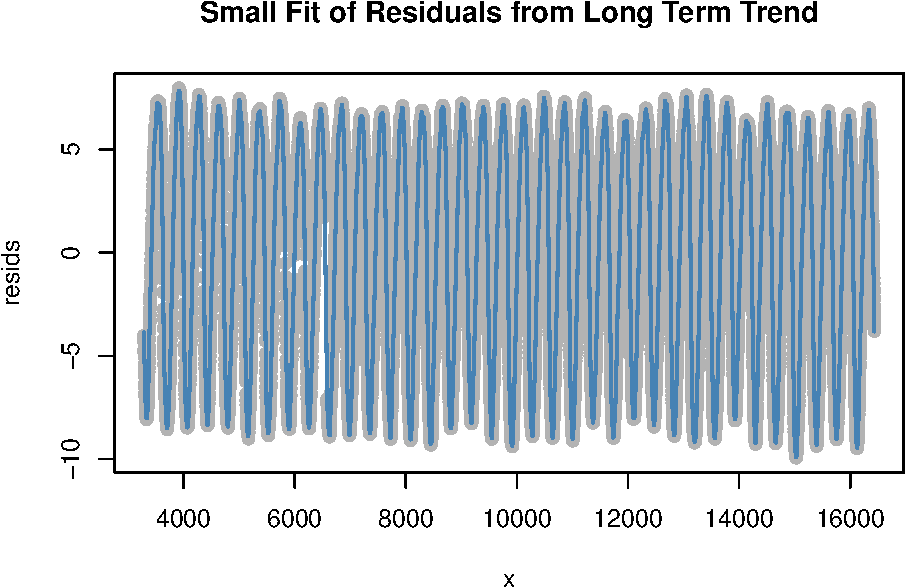
\includegraphics{a4_q3_files/figure-latex/unnamed-chunk-7-1} \end{center}

The residuals exhibit a consistently seasonal trend - it trends upward
and the downwards very quickly for about every \(333\frac{1}{3}\) units
of x, staying with the range of about \([-10, 10]\).

\item 

\textbf{(3 marks)} Plot the residuals from the short-term trend.
Describe any patterns you find.

\begin{Shaded}
\begin{Highlighting}[]
\NormalTok{smresids =}\StringTok{ }\NormalTok{smfit}\OperatorTok{$}\NormalTok{residuals}
\KeywordTok{plot}\NormalTok{(x, smresids, }\DataTypeTok{col=}\StringTok{"grey70"}\NormalTok{, }\DataTypeTok{pch=}\DecValTok{19}\NormalTok{, }
     \DataTypeTok{main=}\StringTok{"Remaining residuals on x"}\NormalTok{)}
\NormalTok{rfit =}\StringTok{ }\KeywordTok{loess}\NormalTok{(smresids}\OperatorTok{~}\NormalTok{x, }\DataTypeTok{span=}\DecValTok{1}\OperatorTok{/}\NormalTok{(}\DecValTok{36}\OperatorTok{*}\DecValTok{12}\NormalTok{))}
\NormalTok{rpred =}\StringTok{ }\KeywordTok{predict}\NormalTok{(rfit)}
\KeywordTok{lines}\NormalTok{(x[xord], rpred[xord], }\DataTypeTok{lwd=}\DecValTok{2}\NormalTok{, }\DataTypeTok{col=}\StringTok{"steelblue"}\NormalTok{)}
\end{Highlighting}
\end{Shaded}

\begin{center}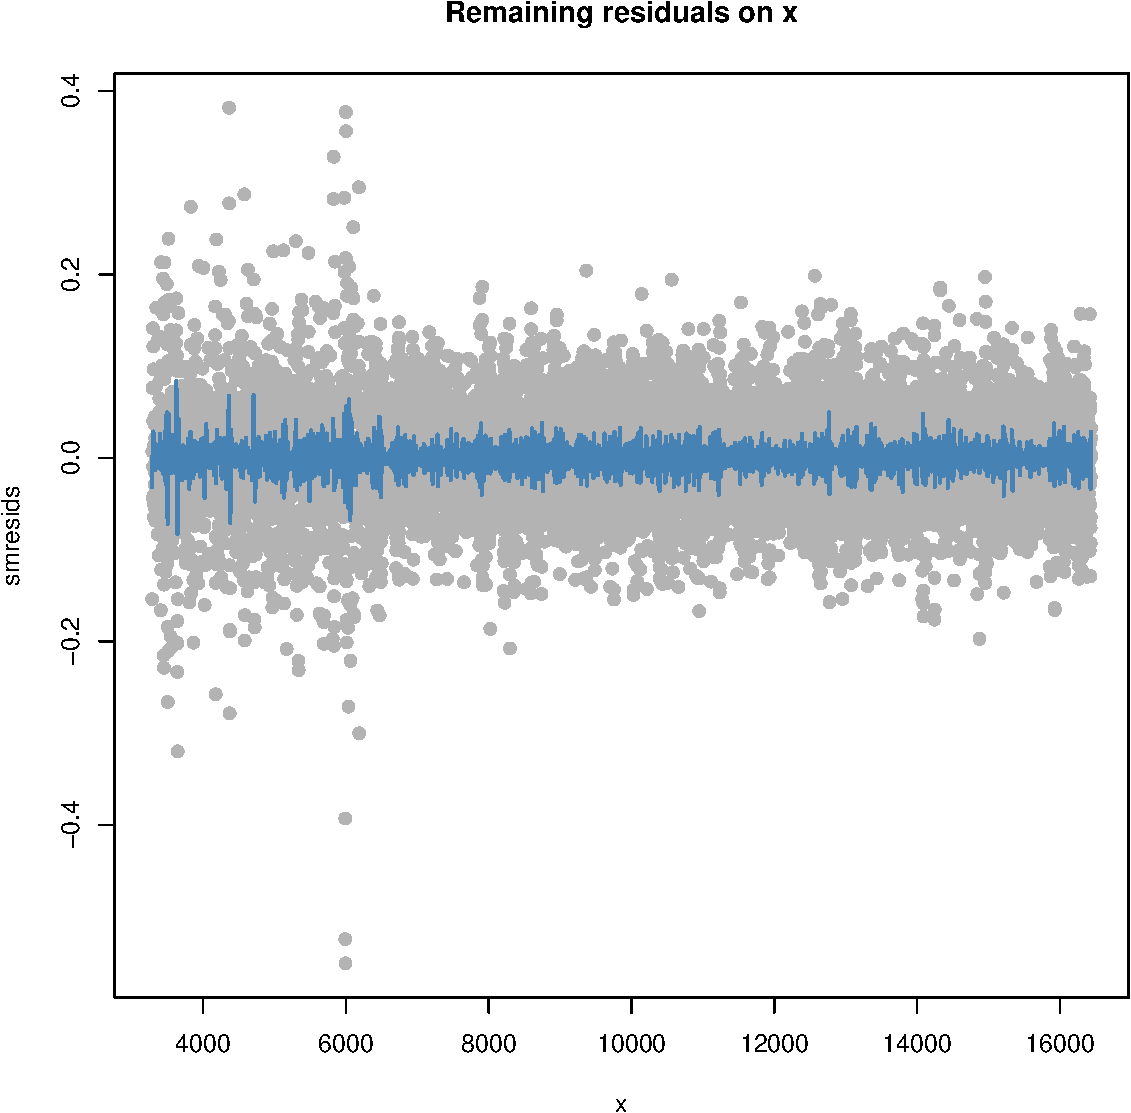
\includegraphics{a4_q3_files/figure-latex/unnamed-chunk-8-1} \end{center}

There is no consistent trend in the plot - the remaining residuals are
too random to locate such a distinct pattern.

\item 

\textbf{(2 marks)} Explain your findings.

The graphs represent the different parts of the decomposition of the
time series model of the Antartic sea ice extent, with the first long
term trend of the extent being the main trend in the model, the short
term trend of the residuals representing the seasonality of the model,
and the remaining residuals representing the remaining randomness in the
model.

\eitem
\eenum

\item 

\textbf{Monthly averages} The original series was very irregular. Here
we replace it with a complete series using the average extent for each
month. This time series is created as follows.

\begin{Shaded}
\begin{Highlighting}[]
\NormalTok{months <-}\StringTok{ }\KeywordTok{unique}\NormalTok{(seaice}\OperatorTok{$}\NormalTok{Month)}
\NormalTok{nmonths <-}\StringTok{ }\KeywordTok{length}\NormalTok{(months)}
\NormalTok{years <-}\StringTok{ }\KeywordTok{unique}\NormalTok{(seaice}\OperatorTok{$}\NormalTok{Year)}
\NormalTok{nyears <-}\StringTok{ }\KeywordTok{length}\NormalTok{(years)}
\CommentTok{# check the beginning and the end months.}
\NormalTok{seaice[}\DecValTok{1}\NormalTok{,]}
\end{Highlighting}
\end{Shaded}

\begin{verbatim}
##   Year Month Day Extent
## 1 1979     1   2  6.945
\end{verbatim}

\begin{Shaded}
\begin{Highlighting}[]
\NormalTok{seaice[}\KeywordTok{nrow}\NormalTok{(seaice),]}
\end{Highlighting}
\end{Shaded}

\begin{verbatim}
##       Year Month Day Extent
## 11552 2014    12  31  9.508
\end{verbatim}

\begin{Shaded}
\begin{Highlighting}[]
\NormalTok{maxN <-}\StringTok{ }\NormalTok{nmonths }\OperatorTok{*}\StringTok{ }\NormalTok{nyears}
\CommentTok{# place holder}
\NormalTok{iceMonthly <-}\StringTok{ }\KeywordTok{vector}\NormalTok{(}\StringTok{"numeric"}\NormalTok{, }\DataTypeTok{length=}\NormalTok{maxN)}
\ControlFlowTok{for}\NormalTok{ (i  }\ControlFlowTok{in} \DecValTok{1}\OperatorTok{:}\NormalTok{nyears) \{}
\NormalTok{  year <-}\StringTok{ }\NormalTok{seaice[,}\StringTok{"Year"}\NormalTok{] }\OperatorTok{==}\StringTok{ }\NormalTok{years[i]}
\NormalTok{  iceyear <-}\StringTok{ }\NormalTok{seaice[year,}\KeywordTok{c}\NormalTok{(}\StringTok{"Month"}\NormalTok{,}\StringTok{"Extent"}\NormalTok{)]}
  \ControlFlowTok{for}\NormalTok{ (j }\ControlFlowTok{in} \DecValTok{1}\OperatorTok{:}\NormalTok{nmonths) \{}
\NormalTok{    index <-}\StringTok{ }\NormalTok{(i}\OperatorTok{-}\DecValTok{1}\NormalTok{) }\OperatorTok{*}\StringTok{ }\NormalTok{nmonths }\OperatorTok{+}\StringTok{ }\NormalTok{j}
\NormalTok{    selection <-}\StringTok{  }\NormalTok{iceyear[,}\StringTok{"Month"}\NormalTok{] }\OperatorTok{==}\StringTok{ }\NormalTok{months[j]}
\NormalTok{    iceMonthly[index] <-}\StringTok{ }\KeywordTok{mean}\NormalTok{(iceyear[selection,}\StringTok{"Extent"}\NormalTok{])}
\NormalTok{  \}}
\NormalTok{\}}
\CommentTok{#  Now we create a time series object}
\NormalTok{ice <-}\StringTok{ }\KeywordTok{ts}\NormalTok{(iceMonthly, }\DataTypeTok{start=}\KeywordTok{c}\NormalTok{(}\DecValTok{1979}\NormalTok{,}\DecValTok{1}\NormalTok{), }\DataTypeTok{frequency=}\DecValTok{12}\NormalTok{)}
\end{Highlighting}
\end{Shaded}

Conduct a seasonal trend analysis on \texttt{ice} using the built-in
\texttt{stl(...)} function with parameters \texttt{s.window=11},
\texttt{s.degree=1}, and \texttt{t.degree=1}.

\benum
\item \textbf{(3 marks)} Plot the output of \texttt{stl} and describe
your findings.

\begin{Shaded}
\begin{Highlighting}[]
\KeywordTok{plot}\NormalTok{(}\KeywordTok{stl}\NormalTok{(ice, }\DataTypeTok{s.window=}\DecValTok{11}\NormalTok{,}
         \DataTypeTok{s.degree=}\DecValTok{1}\NormalTok{, }\DataTypeTok{t.degree=}\DecValTok{1}\NormalTok{))}
\end{Highlighting}
\end{Shaded}

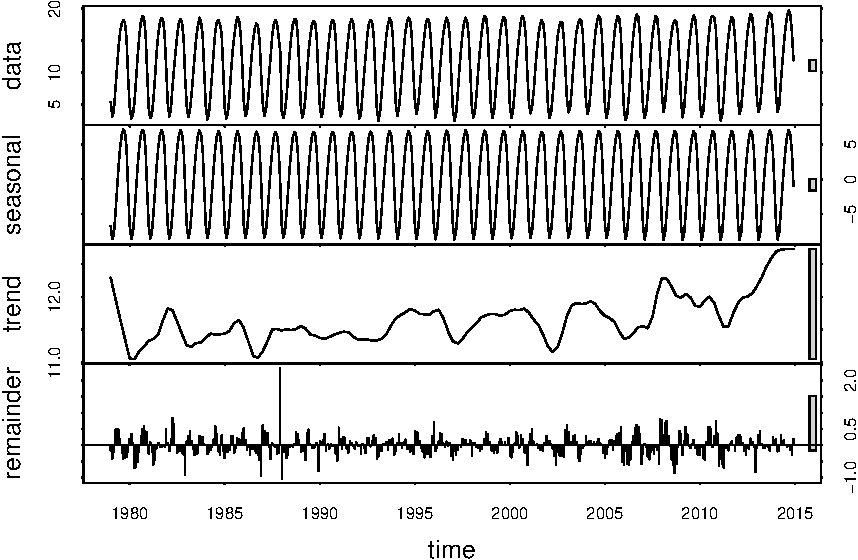
\includegraphics{a4_q3_files/figure-latex/unnamed-chunk-10-1.pdf}

The long term trend of the data is cyclical - the short-term
trends/cycles where the extent decreases and the increases again don't
repeat regularly.

\item 

\textbf{(2 marks)} Compare the output above with the decomposition of
the irregular time series in part (a).

The shape of the seasonal portion of the diagram and randomness of the
remainder is consistent with what was plotted in part (a) for the short
term smooth of residuals and the plot of the remaining residuals
respectively.

However, the main trend of the two questions are different, with the
trend in part (a) having exhibited a stationary trend and the trend in
part (b) being more cyclical. This is due to the irregularity of the
data used in part (a), with part (b) showing the true trend of the data
as the ice extents for the missing dates in part (a) have been accounted
for.

\eenum
\eenum

\eenum


\end{document}
